\chapter{Propuesta de Implementación}\label{chapter:proposal}

Este capítulo detalla la solución computacional propuesta para la generación automática de reportes. Esta propuesta aborda la necesidad de integrar la capacidad generativa de los Modelos de Lenguaje Grandes (LLMs) con la precisión y estructura de la información contenida en bases de conocimiento, ofreciendo un proceso completo desde la interpretación de consultas en lenguaje natural hasta la producción de reportes coherentes, informativos y contextualmente relevantes. La estrategia se centra en el uso de modelos de lenguaje de código abierto, priorizando la accesibilidad, flexibilidad y transparencia. La arquitectura modular de la solución facilita su adaptación y extensión a diversos escenarios y dominios.

\section{Propuesta}

\subsection{Extracción y Selección de Contenido Relevante}

El proceso de generación de reportes se inicia con la interpretación de la consulta del usuario, tarea central que en esta propuesta se delega al Modelo de Lenguaje Grande (LLM). En lugar de recurrir a técnicas tradicionales de Procesamiento del Lenguaje Natural (PLN) para un análisis sintáctico y semántico inicial, se aprovecha la capacidad inherente del LLM para comprender el lenguaje natural, desambiguar la consulta y extraer la intención subyacente del usuario. A partir de esta interpretación, el LLM no solo identifica los conceptos clave y parámetros de búsqueda, sino que también se le solicita generar un esqueleto preliminar del reporte.

Este esqueleto actúa como una estructura guía, dividiendo la consulta original en puntos temáticos o secciones lógicas que abordarán la respuesta final. Una vez definido este esqueleto, la generación de consultas se realiza de forma individual para cada punto temático. Utilizando nuevamente las capacidades del LLM, se formulan consultas específicas y contextualizadas para cada sección del esqueleto, optimizando la extracción de información relevante y garantizando que la respuesta final sea coherente y completa en relación con la consulta original del usuario. Este enfoque nos permite sobrepasar ciertas deficiencias que presenten los LLM en relación al tamaño del contexto que estos sean capaces de manejar.

\subsection{Generación del Reporte}

La información relevante recuperada en la etapa anterior es ahora la base para la generación del reporte. Esta información, que puede estar en forma de tablas, texto o datos estructurados, es organizada y formateada de forma comprensible para un LLM. La pieza central de esta etapa es el diseño del prompt. Se utilizarán técnicas de prompt engineering que incluyen la descomposición de tareas complejas en subtareas más pequeñas y el uso de ejemplos (few-shot learning) para guiar al LLM. El prompt contendrá instrucciones detalladas sobre el estilo, el tono y la estructura deseada del reporte. Además, el prompt especificará la necesidad de incorporar la información extraída de la base de datos, de forma precisa y coherente.

El proceso es iterativo y experimental, y se explorarán diferentes tipos de prompts para optimizar la calidad de la generación, incluyendo estrategias como ``chain-of-thought prompting`` para estimular el razonamiento del LLM antes de generar el reporte final. Se explorarán diversas estrategias de control, como ``constraint prompting`` y ``fact-checking prompting``, que le indiquen al LLM el límite de los hechos o datos verificados por la base de conocimiento, y se eviten las alucinaciones.

\subsection{Uso de Modelos de Lenguaje Open-Source}

La propuesta se basa en el uso de modelos de lenguaje de código abierto, lo que permite una mayor flexibilidad, personalización y reducción de costos. Esta decisión estratégica busca evitar la dependencia de plataformas y modelos cerrados, promoviendo la transparencia y la reproducibilidad de la investigación. Los modelos de lenguaje que se consideran incluyen aquellos pertenecientes a la familia T5 (Text-to-Text Transfer Transformer), LLaMA (Large Language Model Meta AI) y OPT (Open Pre-trained Transformer), entre otros. Estos modelos se han destacado por su desempeño en diversas tareas de procesamiento del lenguaje natural y por su disponibilidad pública.

La selección del modelo específico se realizará en función de su rendimiento en la generación de reportes, su capacidad para trabajar con la información recuperada, y los recursos disponibles para su ajuste y puesta en marcha. Se pretende realizar un ajuste fino (fine-tuning) de los modelos seleccionados, usando datos de ejemplo y técnicas de aprendizaje por refuerzo para optimizar su desempeño en la tarea específica de generación de reportes a partir de bases de conocimiento.

\subsection{Evaluación del Sistema Propuesto}

La evaluación del sistema propuesto es una fase crítica para garantizar su efectividad y validez. Para esto, se llevará a cabo un estudio de caso en un dominio específico, que se definirá de acuerdo con los objetivos del proyecto y la disponibilidad de datos. La evaluación tendrá un enfoque mixto, combinando métricas cuantitativas y cualitativas. Las métricas cuantitativas se basarán en los enfoques clásicos de la evaluación de generación de texto, como BLEU, ROUGE y METEOR, pero se adaptarán para reflejar la relevancia y la precisión de la información extraída de la base de conocimiento y la calidad de la narrativa generada. 

Se introducirán métricas específicas para evaluar la coherencia semántica del reporte, la completitud de la información, y la calidad de la integración de datos y texto. La evaluación cualitativa se realizará a través de la revisión del reporte generado por LLM de mayor nivel y complejidad como GPT-4 y Gemini y por usuarios potenciales, que aportarán retroalimentación valiosa sobre la utilidad, la claridad, y la relevancia del contenido. El análisis de los datos obtenidos de la evaluación permitirá identificar áreas de mejora y refinar la propuesta.


\subsection{Contribuciones Esperadas}

Esta propuesta aspira a contribuir al campo de la generación automática de reportes mediante la combinación de diversas técnicas y enfoques. Primero, se presenta una metodología que logra integrar de forma efectiva la capacidad de los LLMs para la generación de texto con la información extraída de bases de datos. Esta integración permite superar las limitaciones de los enfoques tradicionales de generación de reportes, y al mismo tiempo, intentar disminuir la tendencia de los LLMs a generar información errónea o alucinaciones.

Segundo, la propuesta desarrolla una estrategia de prompt engineering más sofisticada, que ofrece mayor control sobre el contenido, el estilo, y la coherencia de los reportes generados. Tercero, el uso de una base tecnológica open-source democratiza el acceso a la tecnología, haciendo más fácil su adopción y adaptación por parte de la comunidad de investigadores. Cuarto, el proyecto se propone el desarrollo de una metodología de evaluación que, más allá de las métricas tradicionales, se centre en la coherencia, la completitud, la relevancia y la utilidad de los reportes generados. La propuesta sienta las bases para el desarrollo de sistemas de generación automática de reportes más eficaces, flexibles, y transparentes.

\section{Detalles de Implementación}\label{chapter:implementation}

En este capítulo se detalla la implementación de la solución propuesta para la generación automatizada de reportes, describiendo la arquitectura del sistema, los componentes clave y el flujo de trabajo seguido.  Además, se exponen las decisiones de diseño, la selección de herramientas y tecnologías, y se proponen posibles experimentos futuros para evaluar el rendimiento y las capacidades del sistema.

\begin{figure}
	\centering
	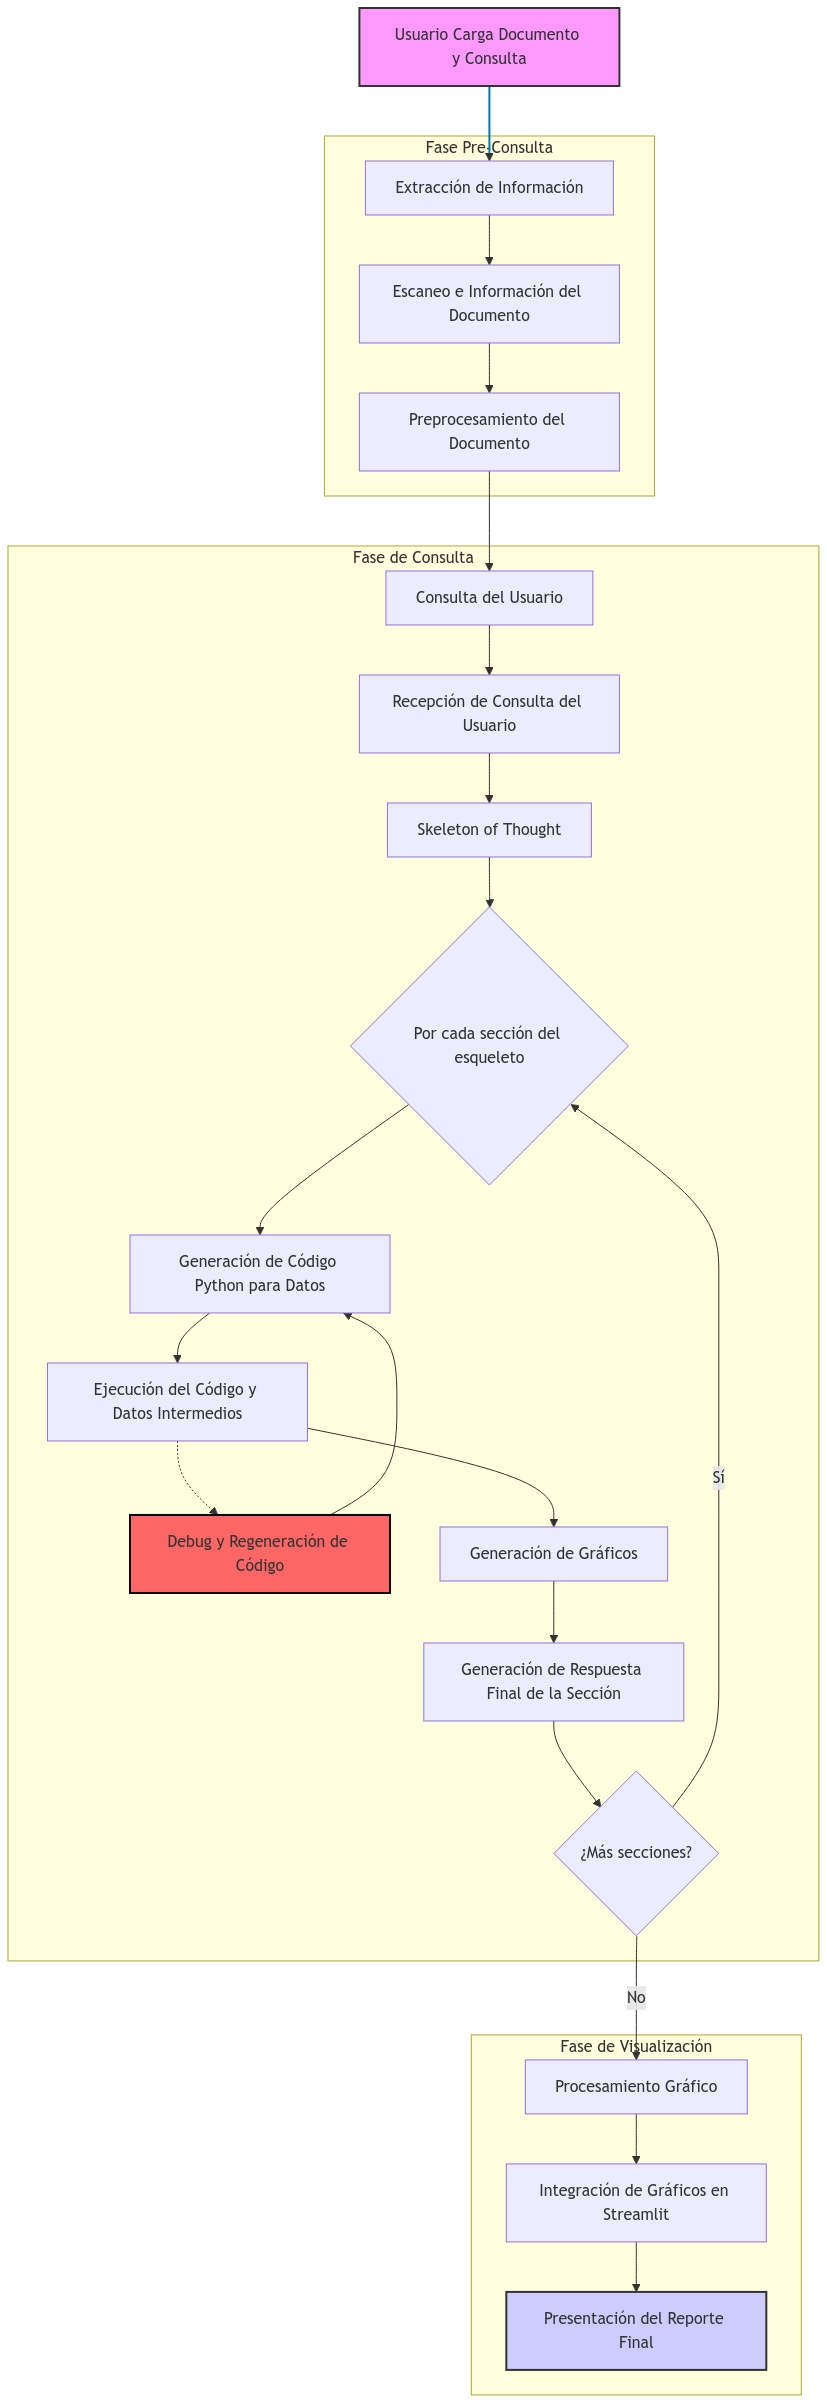
\includegraphics[height=\textheight]{Graphics/graph.png}
	\caption{Flujo de trabajo}
\end{figure}

\subsection{Arquitectura del Sistema y Flujo de Trabajo}

La arquitectura del sistema propuesto se ha diseñado siguiendo un enfoque modular, facilitando la extensibilidad y adaptabilidad a diferentes requerimientos. El flujo de trabajo se divide en etapas claramente definidas, desde la carga del documento por parte del usuario hasta la presentación del reporte final enriquecido con gráficos para una mejor visualización de los resultados. Las etapas principales se pueden categorizar en fases previas a la consulta del usuario, procesamiento de la consulta, y generación de la respuesta y visualización.

\subsubsection{Interfaz Gráfica de Usuario (GUI) con Streamlit}

La interfaz gráfica de usuario se ha construido utilizando la librería Streamlit \cite{streamlit}.  Streamlit se seleccionó por su facilidad de uso,  rapidez de desarrollo y la capacidad de crear interfaces web interactivas y de alta calidad con un mínimo de código Python.  Las características de Streamlit aprovechadas en esta implementación incluyen:

\begin{itemize}
	\item \textbf{Componentes interactivos:}  Streamlit proporciona una amplia gama de componentes interactivos (botones, sliders, áreas de texto, selectores de archivos, checkboxes, etc.) que facilitan la creación de interfaces de usuario dinámicas y receptivas.
	\item \textbf{Renderización de código Altair:}  Streamlit integra la capacidad de renderizar gráficos generados con la librería Altair directamente en la interfaz web,  facilitando la visualización de datos.
	\item \textbf{Desarrollo rápido y iterativo:}  Streamlit permite un ciclo de desarrollo rápido e iterativo.  Los cambios en el código Python se reflejan automáticamente en la interfaz web al guardar el archivo,  agilizando la experimentación y el prototipado.
	\item \textbf{Comunidad activa y documentación extensa:}  Streamlit cuenta con una comunidad de usuarios activa y una documentación completa,  lo que facilita la resolución de problemas y el aprendizaje de nuevas funcionalidades.
\end{itemize}
La interfaz web desarrollada con Streamlit proporciona una experiencia de usuario intuitiva y facilita la interacción con el sistema de generación automatizada de reportes.

\subsubsection{Modelos de Lenguaje Utilizados: API de Groq}

La elección del modelo de lenguaje para esta implementación se basó en la premisa de la limitación de recursos computacionales locales para ejecutar modelos de lenguaje de gran escala con un rendimiento adecuado.  En consecuencia,  se optó por utilizar una API gratuita que proporciona acceso gratuito a modelos open-source de alto rendimiento: la API de Groq\cite{groq}.

La API de Groq ofrece acceso a una variedad de modelos open-source punteros,  incluyendo:

\begin{itemize}
	\item \textbf{gemma2-9b-it (Google):}  Modelo de lenguaje desarrollado por Google,  conocido por su eficiencia y buen rendimiento en diversas tareas con un consumo relativamente bajo de recursos.
	\item \textbf{Familia Llama (Meta):}  Varios modelos de la familia Llama,  desarrollados por Meta (anteriormente Facebook),  incluyendo versiones como Llama 2 y Llama 3.  Se destaca el modelo \textbf{llama-3.3-70b} por sus capacidades demostradas en diversas evaluaciones\cite{llamavsgpt4}.
	\item \textbf{Mixtral-8x7b (Mixtral AI):}  Modelo desarrollado por Mixtral AI,  que ha mostrado un rendimiento competitivo en benchmarks y destaca por su arquitectura Mixture-of-Experts.
\end{itemize}

La utilización de la API de Groq permite experimentar y comparar el rendimiento de diferentes modelos open-source en la tarea de generación de reportes automatizados,  sin requerir una infraestructura computacional local costosa. En futuras investigaciones,  se podría ampliar la experimentación a otros modelos disponibles en la API de Groq o en otras plataformas,  así como explorar estrategias de fine-tuning de los modelos para optimizar su rendimiento en esta tarea específica.


\subsection{Fases Previas a la Consulta del Usuario}

Esta fase inicial se centra en la preparación del entorno y el procesamiento preliminar del documento proporcionado por el usuario. Esta fase consta de los siguientes pasos:

\subsubsection{Carga del Documento por el Usuario}

El sistema inicia con la carga del documento por parte del usuario a través de la interfaz web. Se implementa un componente de carga de archivos el cual forma parte de la librería de streamlit y que admite diversos formatos de documento comunes para el análisis de datos, incluyendo:
\begin{itemize}
	\item \textbf{CSV (.csv):}  Formato de valores separados por comas, ampliamente utilizado para datos tabulares.
	\item \textbf{Excel (.xlsx):}  Formato de hoja de cálculo de Microsoft Excel, capaz de almacenar datos tabulares y fórmulas complejas.
	\item \textbf{Texto (.txt):}  Formato de texto plano, aunque su soporte es más limitado en la implementación actual y se centra en la extracción de información general del documento para contextualizar al LLM.  [Se podría ampliar el soporte para documentos de texto en futuras iteraciones, implementando técnicas de segmentación y análisis semántico más robustas.]
\end{itemize}

La flexibilidad en los formatos de entrada busca maximizar la accesibilidad y usabilidad del sistema para usuarios con diferentes tipos de datos.

\subsubsection{Escaneo e Información del Documento}

Una vez cargado el documento, se procede a un análisis inicial para extraer información relevante que se proporcionará al LLM en etapas posteriores. La función ``get\_document\_info`` se encarga de este proceso, adaptándose al tipo de documento cargado.  Para documentos tabulares (CSV, Excel, JSON), se utiliza la librería Pandas para cargar los datos en un DataFrame, debido a la gran cantidad de funciones que posee esta librería para un mejor control y análisis de los datos. Esta información que se busca extraer del documento en cuestión se busca que sea lo más corta pero relevante posible ya que debe servir de base para que un LLM tenga una idea del documento en cuestión y como realizar consultas sobre este.

Este enfoque busca emular el comportamiento que seguimos al enfrentarnos a un conjunto de datos que del cual no tenemos información previa. Nosotros como humanos hacemos lo mismo cuando nos enfrentamos a un gran volumen de datos, solo miramos los nombres de las columnas y quizás un par de filas para tener una idea de los tipos de datos con los que estamos trabajando. 

La información extraída incluye:

\begin{itemize}
	\item \textbf{Nombres de las columnas:}  Se obtienen los nombres de las columnas del DataFrame, proporcionando al LLM el vocabulario básico de los datos.
	\item \textbf{Tipos de las columnas:}  Se identifican los tipos de datos de cada columna (numérico, categórico, fecha, etc.),  lo cual es crucial para que el LLM genere código de procesamiento adecuado.
	\item \textbf{Valores Mínimos y Máximos por columna (numéricas):} Se calculan los valores mínimo y máximo para cada columna numérica, ofreciendo al LLM una idea del rango y escala de los datos.
	\item \textbf{Cantidad de Valores Únicos por columna:} Se determina el número de valores únicos en cada columna, lo que puede indicar si una columna es categórica o numérica continua.
	\item \textbf{Valores Faltantes por columna:} Se cuantifica la cantidad de valores faltantes (NaN) en cada columna, información relevante para que el LLM considere estrategias de imputación o manejo de datos faltantes si es necesario.
	\item \textbf{Valores de las primeras filas:} Se muestran las primeras filas del DataFrame tal y como vienen para que el LLM determine correctamente como son los datos de cada columna.
\end{itemize}
Esta información se estructura en un diccionario JSON y se almacenan en una variable ``document\_info`` que se utilizará en las interacciones posteriores con el LLM como parte del prompt.

\subsubsection{Preprocesamiento del Documento}

Para una mejor respuesta estadística, y datos más fiables, generalmente se necesita hacer un preprocesamiento de los datos recibidos, ya que estos pueden venir de diferentes fuentes, presentar valores faltantes o algunas inconsistencias en el formato de cada columna. Dicho preprocesamiento puede ser completamente basado en reglas, completamente basado en LLM, o un enfoque híbrido.

El procesamiento basado en reglas especifica que reglas y criterios tener en cuenta a la hora del preprocesamiento, por ejemplo, las reglas pueden dictar que para cierta fila los datos faltantes se rellenen con el valor de la media de la fila o que ciertos valores outliers necesitan ser topados o normalizados. Este método es altamente estructurado y necesita un conocimiento profundo de los datos en cuestión.

El preprocesamiento basado en LLM consiste en utilizar un modelo de lenguaje para rellenar o modificar los datos faltantes asi como categorizar o detectar y corregir inconsistencias en los datos. Utilizando el poder del los LLMs permite manejar datos que en principio no estén bien estructurados así como inferir nuevos datos a partir de texto en lenguaje natural como por ejemplo detectar una valoración de 1-5 basado en un comentario de un usuario.

El problema que presentan estos tipos de preprocesamiento es que vamos a estar trabajando con un conjunto de datos potencialmente muy grande y del cual no se cuenta con información previa, por lo que no podríamos tener reglas predefinidas para las columnas ya que no sabemos que datos se representan en ellas y no podríamos utilizar las capacidades del LLM para el preprocesado dado el limitado contexto que estos presentan.

Es por esto que se decidió utilizar un enfoque híbrido en cuanto al preprocesado, es decir, utilizar las capacidades de generación de código de los LLM y a partir de estas generar las reglas. Construir un preprocesador de este tipo vendría dado por diseñar un sistema que analice un dataset de entrada, y a partir de este entienda que transformaciones y reglas debe seguir para producir el dataset de salida deseado.

La función ``preprocess\_document`` es la encargada de este proceso, y se divide en dos etapas principales:

\begin{enumerate}
	\item \textbf{Definición de Tareas de Preprocesamiento por el LLM:} Se formula un prompt al LLM solicitándole que analice la información del DataFrame con la información del documento que habíamos recolectado anteriormente y sugiera tareas de preprocesamiento relevantes.  El prompt especifica que la respuesta debe ser en formato JSON,  conteniendo una lista de diccionarios, cada uno representando una tarea con detalles como el tipo de tarea, la columna afectada y parámetros adicionales (por ejemplo, formato de fecha).  Las tareas consideradas en el prompt incluyen:
	\begin{itemize}
		\item \textbf{Conversión de Fechas:}  Identificación de columnas que contienen fechas y sugerencia de conversión al tipo `datetime` de Pandas, especificando el formato de fecha si es necesario.
		\item \textbf{Identificación de Columnas Categóricas:}  Reconocimiento de columnas con un número limitado de valores únicos que podrían ser tratadas como variables categóricas.
		\item \textbf{Sugerencias para Columnas No Numéricas No Categóricas:}  Detección de columnas no numéricas que no parecen ser categóricas y sugerencias para su filtrado o tratamiento (e.g., columnas de texto libre que no son relevantes para el análisis numérico).
	\end{itemize}
	
	\item \textbf{Ejecución de Tareas de Preprocesamiento:}  Se itera sobre la lista de tareas de preprocesado que generó el LLM y se genera código Python dinámicamente para cada tarea.  Este código se ejecuta utilizando la función ``execute\_code``, la cual sirve para ejecutar el código en un entorno seguro y controlado, pasando el DataFrame `df`. El comportamiento de esta función se detalla más adelante.
\end{enumerate}

\subsection{Fase de Procesamiento de la Consulta del Usuario}

Una vez que el documento ha sido cargado y preprocesado, el sistema está listo para recibir y procesar las consultas del usuario. Esta fase se compone de los siguientes pasos:

\subsubsection{Recepción de la Consulta del Usuario}

El usuario introduce su consulta en lenguaje natural a través de un área de texto en la interfaz web. Esta consulta representa la pregunta o solicitud de información que el usuario desea obtener a partir del documento cargado.

\subsubsection{Skeleton of Thought: Descomposición del Reporte a Generar}

Se implementa la estrategia ``Skeleton of Thought`` para abordar la complejidad de las consultas.  En lugar de intentar generar una respuesta directa,  se solicita al LLM que a partir de la consulta del usuario genera la estructura o ``esqueleto`` del reporte a generar, para esto se le provee al modelo los siguientes datos en el ``prompt``.

\begin{itemize}
	\item \textbf{La consulta del usuario en lenguaje natural.}
	\item \textbf{Información relevante sobre el DataFrame (proveniente de ``document\_info``).}
	\item \textbf{Instrucciones claras sobre el formato de respuesta esperado:}  Se indica al LLM que debe responder con un breve análisis de la consulta y una lista de secciones delimitadas dentro de un fragmento de código json. Donde cada sección se le pide que genere los siguientes datos para un mayor control posterior de la sección. 
	\begin{itemize}
		\item \texttt{'name'}: - Nombre descriptivo de la sección.
		\item \texttt{'description'}: -  Explicación concisa del propósito de la sección.
		\item \texttt{'data'}: - Descripción del tipo de información que contendrá la sección.  Indicar si se requieren visualizaciones (gráficos, tablas) y sugerir tipos apropiados (ej: ``Gráfico de barras para comparar ventas``, ``Tabla con datos numéricos detallados``).
		\item \texttt{'extra\_data'}: -  Sugerencias de información adicional que podría enriquecer la sección y aportar valor al usuario.
	\end{itemize}
\end{itemize}

La respuesta del LLM, que contiene el análisis y la lista de secciones,  se almacena como ``skeleton\_response`` y se muestra en la interfaz web para la revisión del usuario en caso de tener activado el modo depuración, del cual hablaremos más adelante.

\subsubsection{Generación de Código Python para obtener datos concisos}

Para cada sección identificada en el paso anterior, se solicita al LLM que genere código Python utilizando la librería Pandas para operar sobre el DataFrame $`df`$.  El proceso se repite para cada tarea sección individualmente.  El prompt formulado al LLM en este paso incluye:

\begin{itemize}
	\item \textbf{El nombre, la descripción, y los datos generados en el proceso de creación del esqueleto del reporte.}
	\item \textbf{Información relevante sobre el DataFrame:} proveniente de la variable  ``document\_info``.
	\item \textbf{Instrucciones sobre el formato de respuesta esperado:} Se especifica que el LLM debe responder con código Python encapsulado entre delimitadores.
\end{itemize}
Además se utiliza una técnica llamada ``constraint prompting`` en donde se le restringe las capacidades generativas del LLM a seguir una serie de reglas, en este caso se le pide que el código python a generar no puede modificar el dataframe original, que los datos relevantes que desee recuperar los debe almacenar en una variable local llamada ``response``, y que no recupere grandes volúmenes de datos, solo la información relevante que sea capaz de extraer usando código python de estos.

La respuesta del LLM, que contiene el código Python se parsea para determinar solamente la región donde se encuentra el código, se almacena como ``code\_response`` y se muestra en la interfaz web en caso de depuración.

\subsubsection{Ejecución del Código y Obtención de Resultados Intermedios}

El código Python generado para cada tarea atómica se ejecuta utilizando nuevamente la función ``execute\_code``.  Esta función ejecuta el código en un entorno seguro,  pasando el DataFrame $`df$` como variable local.  El resultado de la ejecución como se le había pedido al modelo se deben encontrar en la variable local response. Si la ejecución es exitosa,  los resultados (que pueden ser DataFrames, series, valores numéricos, diccionarios, etc.).  Si ocurre un error durante la ejecución,  se captura el error y se muestra en la interfaz web en caso de depuración y  luego se intenta utilizar nuevamente el LLM para corregir el código python en cuestión.

La función ``execute\_code`` contiene un parámetro opcional ``max\_retries``, el cual se utiliza para evitar caer en un ciclo infinito donde no se pueda corregir el código en cuestión. Para intentar arreglar el código se acude nuevamente al modelo del lenguaje, este proceso se realiza mediante la función ``debug\_and\_regenerate\_code``, la cual recibe como parámetros el código que se ejecuto y dio error y el mensaje de error lanzado, y a partir de esos datos se le pide al LLM que genere un nuevo código python, el cual automáticamente se parsea y se vuelve a intentar ejecutar.

\subsubsection{Generación de Gráficos}

Para mejorar la visualización de los datos y la calidad de los reportes se hace necesario la inclusión de elementos gráficos que permitan al usuario ver y entender una mayor cantidad de datos y su comportamiento. Para la generación de estos gráficos seguimos la misma idea de el punto anterior de obtención de datos, como no podemos proveer a los LLM con todo el conjunto de datos para que este renderize un gráfico o tabla a partir de esto, lo que hacemos es pedirle que genere código python que sea capaz de generar estos gráficos.

Para este propósito utilizamos la librería altair\cite{altair}, una librería capaz de generar varios tipos de gráficos a partir de un dataframe en pandas, estas facilidades unidos a la funcionalidad de streamlit de renderizar dichos gráficos directamente en la web con una sola intrucción, hacen de esta librería una opción ideal para este trabajo.

En este paso se siguen las mismas ideas, en cuanto a la estructura del prompt, que las vistas en la sección \textbf{Generación de Código Python para obtener datos concisos}. Con la diferencia que se le hace saber al modelo que la librería altair ya esta importada como ``alt``, y que las respuestas deben ser una lista de diccionarios que contengan la siguiente información:

\begin{itemize}
	\item \textbf{name} :- Nombre del gráfico, este se utiliza luego como un id para acceder al gráfico en cuestión.
	\item \textbf{description} :- Una breve descripción del gráfico en cuestión y los datos que representa para que a la hora de generar la respuesta final a partir de esta información el modelo de lenguaje sepa en que posición ubicarlo.
	\item \textbf{c} :- Referencia al objeto Altair del gráfico.
\end{itemize}

\subsubsection{Generación de la Respuesta Final de la sección}

Para la generación de la sección final del reporte, se recurre al LLM, al cual se le proporciona toda la información procesada y relevante para la sección en cuestión. Esto incluye los datos extraídos y calculados previamente, la información contextual del documento analizado, y las descripciones de las visualizaciones gráficas generadas. Con el objetivo de facilitar la integración de gráficos dentro del flujo textual del reporte, se instruye al LLM para que utilice una sintaxis inspirada en markdown. Específicamente, se le indica que inserte un bloque de código ```chart <nombre\_del\_gráfico> ``` en aquellos puntos donde considere pertinente incluir una visualización.

Una vez obtenida la respuesta del LLM, se procede a analizarla (parsearla) para identificar estos marcadores de gráficos. Posteriormente, estos marcadores son reemplazados programáticamente por las correspondientes gráficas generadas con Altair, permitiendo una integración fluida y dinámica de texto y visualizaciones en la sección del reporte final presentada en Streamlit.

